\documentclass[../taasin.tex]{subfiles}
\graphicspath{{\subfix{../figures/}}}
\begin{document}
\label{appendix:linet}

%%%%%%%%%%%%%%%%%%%%%%%%%%%%%%%%%%%%%%%%%%%%%%%%%%%%%%%%%%%%%%%%%%%%%%

% [LiNet appendix?] Fast convergence, biologically reasonable, good performance

Convolutional layers have allowed for great progress in computer vision. They improve upon fully
connected layers, where a neuron in a given layer is connected to all neurons in the previous layer. In CNNs, each neuron is only connected to neighboring units in the previous layer. Of course, this "neighboring" is dependent on the fact that image inputs are organized in structured arrays. Our ONV is an unstructured input and doesn't naturally lend itself to working with CNNs.

This leaves us to experiment with a fully connected architecture. The only problem is that our ONV is a vector of dimension 43,200. A fully connected model created to process this large of a vector would use a great amount of memory and be slow to train. 

The work of \cite{Masaki} solved this by going back to the idea of locally connected networks. Dubbed a "LiNet," each neuron only processes inputs from photoreceptors that are close to each other. The architecture is summarized in figure \ref{fig:linet_rgb}. Furthermore, the number of neurons in each subsequent layer is scaled down by a factor f. The architecture converges very quickly and uses much less memory than a comparable fully connected architecture. In addition, it scales much better to larger numbers of photoreceptors.

\begin{figure}[h]
    \centering
    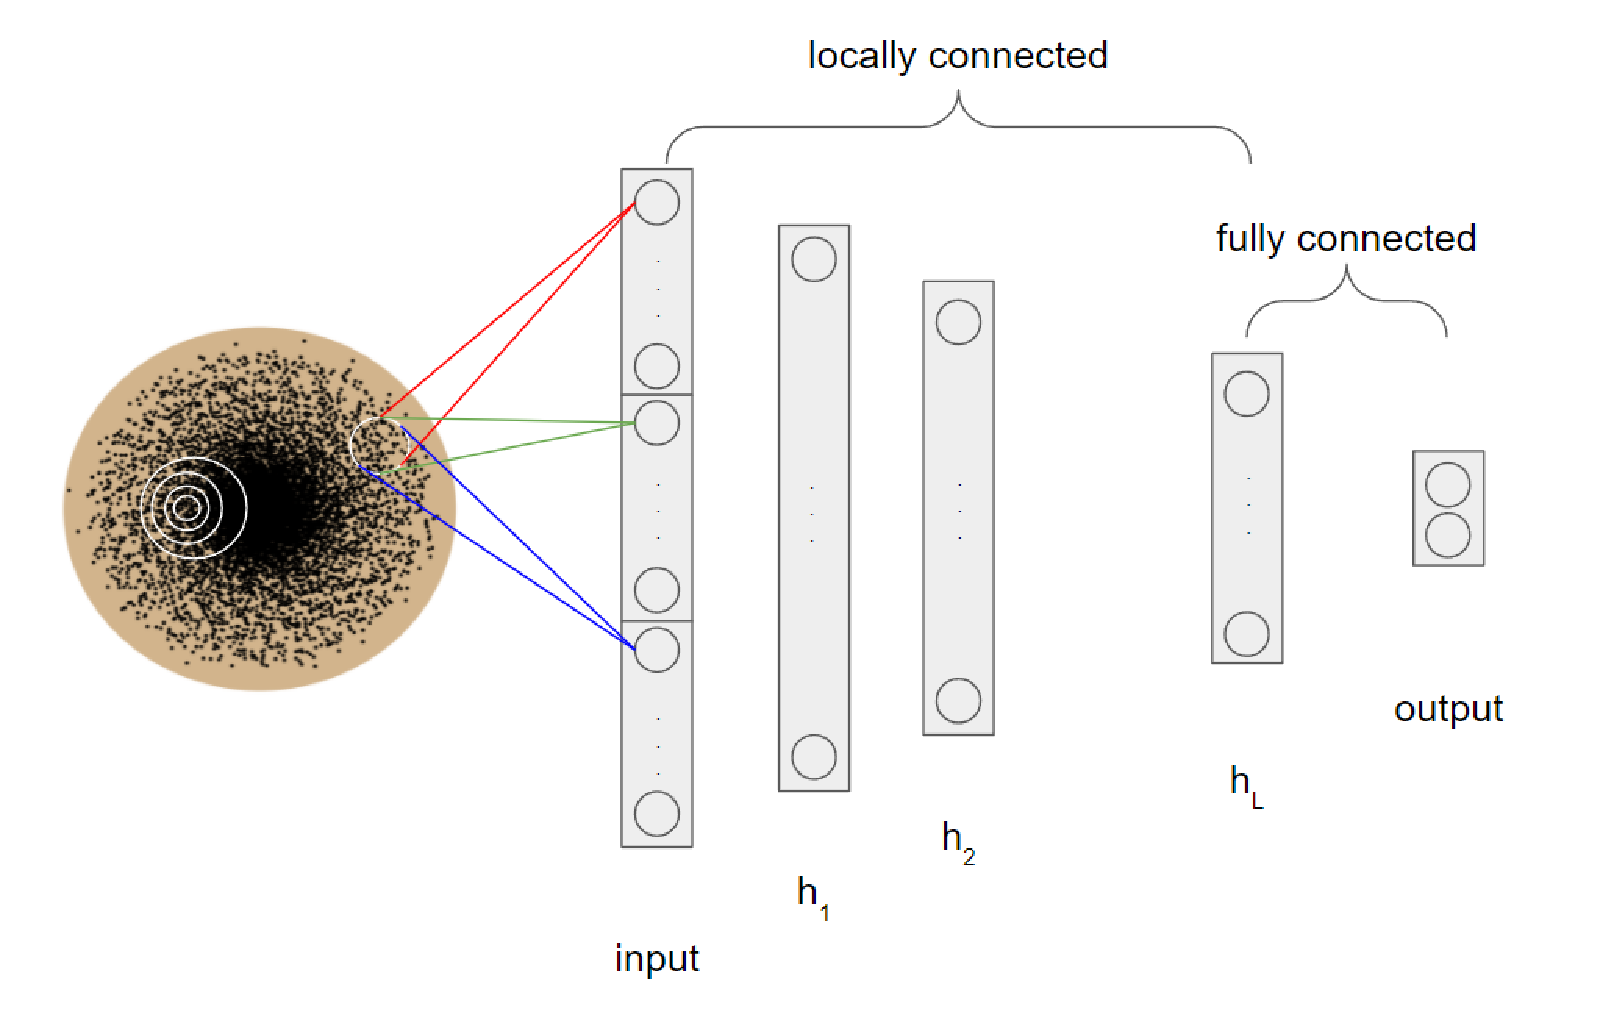
\includegraphics[width=0.5\textwidth]{figures/linet_summary.pdf}
    \caption{The LiNet architecture. We have a 14,400 photoreceptor retina with red, blue and green channels stacked on top of each other to create the ONV. Each neuron then processes the K nearest red, blue, or green inputs to itNeurons at the first layer combine input from a handful of photoreceptors. Neurons in consecutive layers combine the fields of view from previous layers to slowly get closer to seeing the full scene.}
    \label{fig:linet_rgb}
\end{figure}

Figure \ref{fig:linet_receptive_fields} illustrates the advantage of using locally connected networks. The neurons in earlier layers see inputs from a group of neighboring photoreceptors. Neurons in later layers see larger groups of neighboring photoreceptors.

% Image showing neighboring circles getting bigger
% \begin{figure}[h]
%     \centering
%     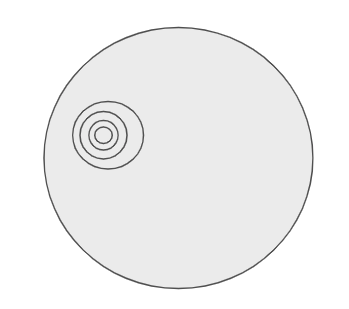
\includegraphics[width=0.5\textwidth]{figures/linet_receptive_fields.png}
%     \caption{}
%     \label{fig:linet_receptive_fields}
% \end{figure}

%%%%%%%%%%%%%%%%%%%%%%%%%%%%%%%%%%%%%%%%%%%%%%%%%%%%%%%%%%%%%%%%%%%%%%

\subsection{Training}

We re-train the LiNet architecture as we did not have access to the previously trained model. We collect data points by randomly sampling positions that the target can take in the eye's field of view. Then, through inverse dynamic simulation, we collect the exact angles needed track the target given the current ONV input. Our dataset consisted of 25 thousand datapoints, 2.5 thousand of which were kept for validation and another 2.5 thousand of which were used for testing. 

We kept the 5 layer architecture reported in the original work. We use a factor $f$ of 5, meaning each subsequent layer has half the number of neurons as the previous layer. A number was not reported for $k$, the number of photoreceptors to group together in the input. We conducted a hyperparameter sweep and use a value of 25.

Training was done with a batch size of 16 and a learning rate of 0.001. No regularization is added to the model, and the weights are inialized with He initialization.

%%%%%%%%%%%%%%%%%%%%%%%%%%%%%%%%%%%%%%%%%%%%%%%%%%%%%%%%%%%%%%%%%%%%%%

\end{document}